\documentclass{article}
\usepackage[top=3cm, bottom=3cm, left = 2cm, right = 2cm]{geometry}
\geometry{a4paper}
\usepackage[T1]{polski}
\usepackage[utf8]{inputenc}
\usepackage{titling}
\usepackage{caption}
\usepackage[parfill]{parskip}
\usepackage{hyperref}
\usepackage{multirow}
\usepackage{graphicx}
\usepackage{tikz}
\usetikzlibrary{decorations.markings}
\usepackage{subcaption}
\usepackage{pgffor}

\renewcommand\maketitlehooka{\null\mbox{}\vfill}
\renewcommand\maketitlehookd{\vfill\null}

\begin{document}

\begin{titlingpage}
    \title{Algorytmy metaheurystyczne\\[1ex] \large Problem komiwojażera euklidesowego. Symulowane Wyżarzanie. Tabu Search.}
    \author{Karol Janic}
    \date{16 grudnia 2023}

    \maketitle
\end{titlingpage}

\tableofcontents

\newpage

\section{Cel zadania}
Celem zadania jest sprawdzenie skuteczności heurystyki symulowanego wyżarzania oraz tabu search na przykładzie euklidesowego problemu komiwojażera oraz
zbadanie wpływu wyboru parametrów tych heurystyk, rozwiązania początkowego i metody generowania otoczenia na jakość rozwiązania.

\section{Opis algorytmów}
\subsection{Symulowane wyżarzanie}
Metaheurystyka polega na przeszukiwaniu przestrzeni rozwiązań w celu znalezienia rozwiązania optymalnego. 
\newline
W każdym kroku algorytmu wybierane jest rozwiązanie z otoczenia aktualnego rozwiązania. Jeżeli rozwiązanie to jest lepsze od aktualnego, to staje się ono aktualnym rozwiązaniem. 
W przeciwnym wypadku, rozwiązanie to staje się aktualnym rozwiązaniem z pewnym prawdopodobieństwem. Prawdopodobieństwo to maleje wraz z upływem czasu poprzez ustalnie aktualnej temperatury, 
która zmniejsza się w czasie. Zatem w początkowej fazie algorytmu prawdopodobieństwo wybrania gorszego rozwiązania jest większe, a w końcowej małe.
\newline
Początkowa temperatura ustalana jest jako $T := \alpha N$, gdzie $N$ to liczba wierzchołków.
Szukanie rozwiązania podzielone jest na epoki o ustalonej liczbie iteracji równej $S := \gamma T$. Po każdej epoce aktualna temperatura jest zmniejszana o ustalony czynnik: $T' := \beta T$.
Rozwiązanie szukane jest do momentu gdy od ustalonej liczby iteracji $M := \delta N$ nie udało się znaleźć lepszego rozwiązania.
\newline
Rozważane są dwa sposoby generowania otoczenia: pełne(sprawdzenie wszystkich sąsiadów) oraz losowe(sprawdzenie $N$ losowych sąsiadów). Rozważanym otoczeniem jest otoczenie \texttt{INVERT}.
Sprawdzane są także dwa sposoby generowania rozwiązania początkowego: losowe oraz oparte o MST.

\subsection{Tabu Search}
Metaheurystyka polega na przeszukiwaniu przestrzeni rozwiązań w celu znalezienia rozwiązania optymalnego. 
\newline
W każdym kroku algorytmu wybierane jest takie rozwiązanie z otoczenia aktualnego rozwiązania
aby było ono najlepsze spośród wszystkich rozwiązań w otoczeniu oraz nie znajdowało się na liście tabu. Jeżeli rozwiązanie to jest lepsze od aktualnego, to staje się ono aktualnym rozwiązaniem.
Każde rozwiązanie dodawane jest do listy tabu na określoną liczbę iteracji. W ten sposób algorytm może wyjść z lokalnego minimum.
\newline
Maksymalna długość listy tabu ustalana jest jako $L := \alpha N$, gdzie $N$ to liczba wierzchołków. Gdy lista tabu jest pełna, to usuwane jest z niej najstarsze rozwiązanie.
Rozwiązanie szukane jest do momentu gdy od ustalonej liczby iteracji $M := \beta N$ nie udało się znaleźć lepszego rozwiązania.
\newline
Rozważane są dwa sposoby generowania otoczenia: pełne(sprawdzenie wszystkich sąsiadów) oraz losowe(sprawdzenie $N$ losowych sąsiadów). Rozważanym otoczeniem jest otoczenie \texttt{INVERT}.
Sprawdzane są także dwa sposoby generowania rozwiązania początkowego: losowe oraz oparte o MST.

\section{Dane testowe}
Opisane wyżej metaheurystyki zostały nastrojone oraz testowane na przykładach z \url{https://www.math.uwaterloo.ca/tsp/vlsi/index.html}.

\section{Strojenie parametrów}
Proces strojenia polegał na sprawdzenie wpływu zmiany poszczególnych parametrów na jakość rozwiązania. Został on przeprowadzony na kilku mniejszych przykładach.
Wykresy poniżej prezentują minimalną wagę cyklu, średnią wagę cyklu oraz średni czas działania heurystyki dla jednej iteracji w zależności od wyboru parametrów.
Zostały one wyznaczone na podstawie 10 uruchomień heurystyki dla każdej kombinacji parametrów.

\newpage

\subsection{Symulowane wyżarzanie}
\subsubsection{Wpływ zmiany temperatury początkowej na średnią długośc cyklu rozwiązania}
    \begin{figure}[h!]
        \centering
        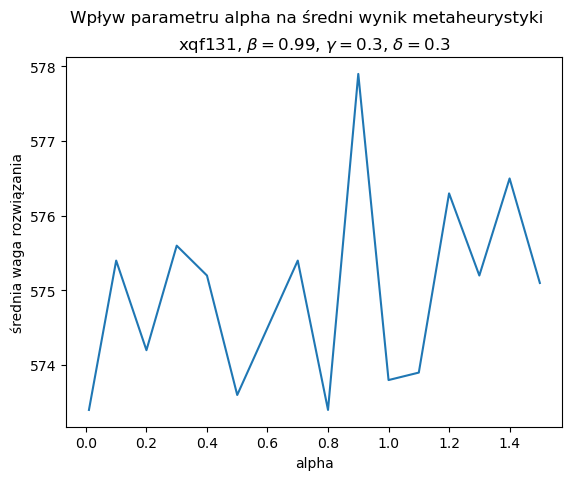
\includegraphics[height=9.5cm]{../../plots/sa-tuning-alpha-avg-xqf131.png}
    \end{figure}

    \begin{figure}[h!]
        \centering
        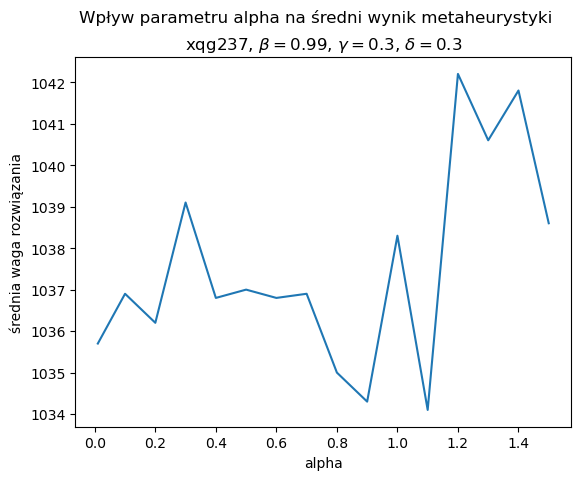
\includegraphics[height=9.5cm]{../../plots/sa-tuning-alpha-avg-xqg237.png}
    \end{figure}

\newpage

\subsubsection{Wpływ zmiany temperatury początkowej na minimalną długośc cyklu rozwiązania}
    \begin{figure}[h!]
        \centering
        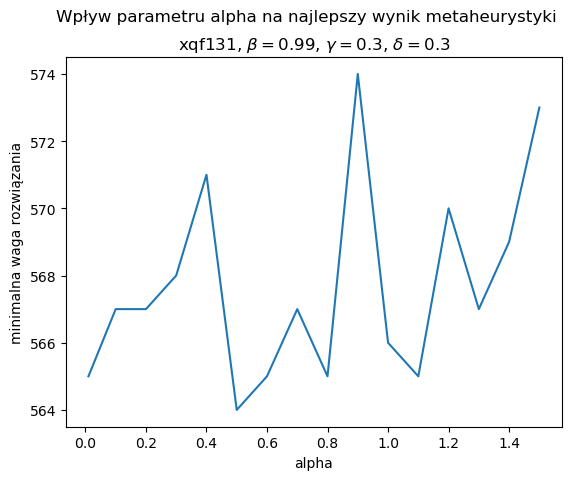
\includegraphics[height=9.5cm]{../../plots/sa-tuning-alpha-min-xqf131.png}
    \end{figure}

    \begin{figure}[h!]
        \centering
        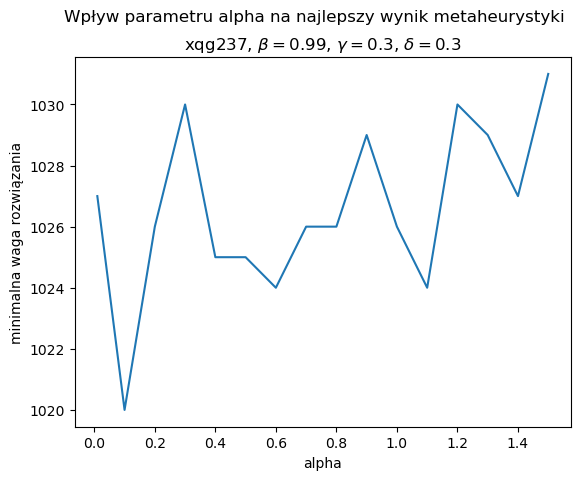
\includegraphics[height=9.5cm]{../../plots/sa-tuning-alpha-min-xqg237.png}
    \end{figure}

\newpage

\subsubsection{Wpływ zmiany temperatury początkowej na średni czas działania heurystyki}
    \begin{figure}[h!]
        \centering
        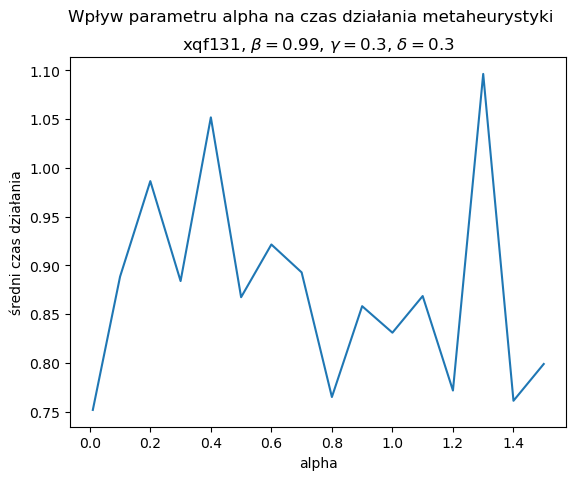
\includegraphics[height=9.5cm]{../../plots/sa-tuning-alpha-time-xqf131.png}
    \end{figure}

    \begin{figure}[h!]
        \centering
        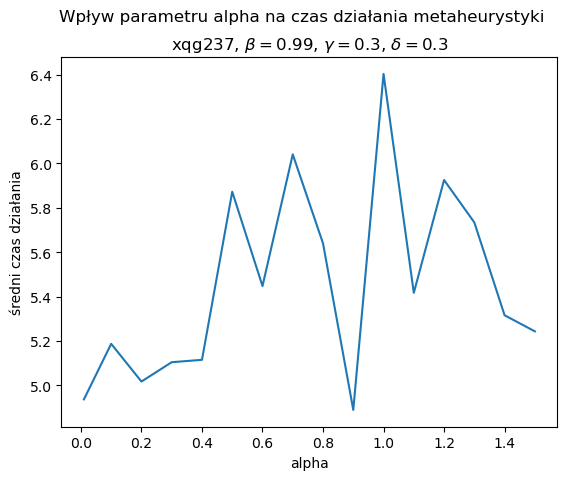
\includegraphics[height=9.5cm]{../../plots/sa-tuning-alpha-time-xqg237.png}
    \end{figure}


\newpage 

\subsubsection{Wpływ zmiany chłodzenia na średnią długośc cyklu rozwiązania}
    \begin{figure}[h!]
        \centering
        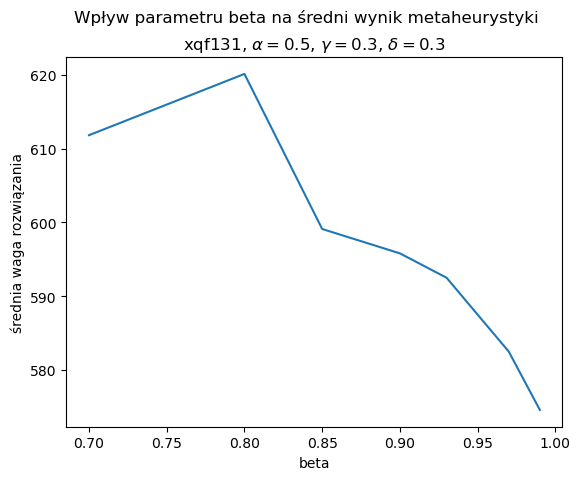
\includegraphics[height=9.5cm]{../../plots/sa-tuning-beta-avg-xqf131.png}
    \end{figure}

    \begin{figure}[h!]
        \centering
        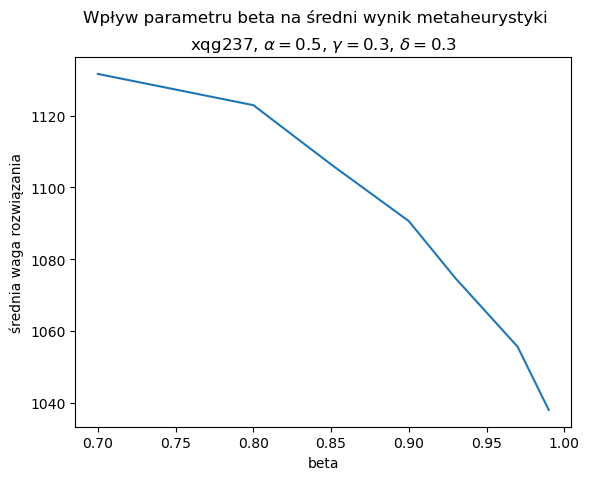
\includegraphics[height=9.5cm]{../../plots/sa-tuning-beta-avg-xqg237.png}
    \end{figure}

\newpage

\subsubsection{Wpływ zmiany chłodzenia na minimalną długośc cyklu rozwiązania}
    \begin{figure}[h!]
        \centering
        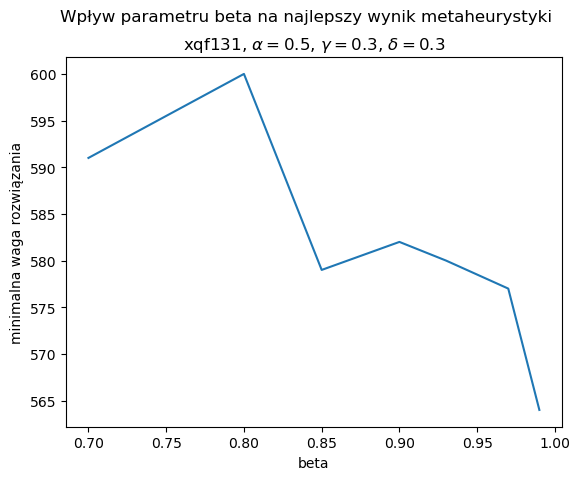
\includegraphics[height=9.5cm]{../../plots/sa-tuning-beta-min-xqf131.png}
    \end{figure}
    
    \begin{figure}[h!]
        \centering
        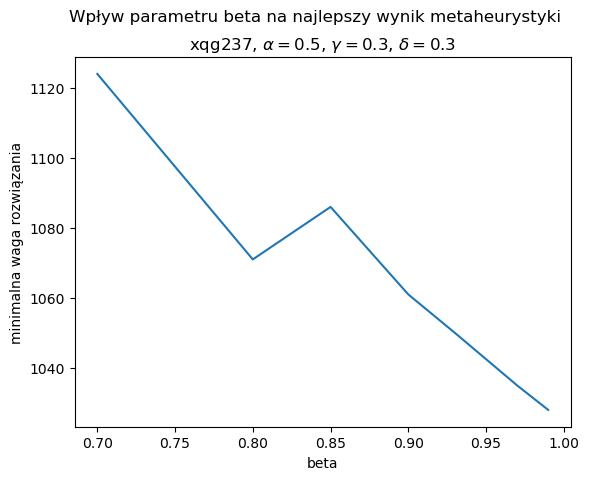
\includegraphics[height=9.5cm]{../../plots/sa-tuning-beta-min-xqg237.png}
    \end{figure}

\newpage

\subsubsection{Wpływ zmiany chłodzenia na średni czas działania heurystyki}
    \begin{figure}[h!]
        \centering
        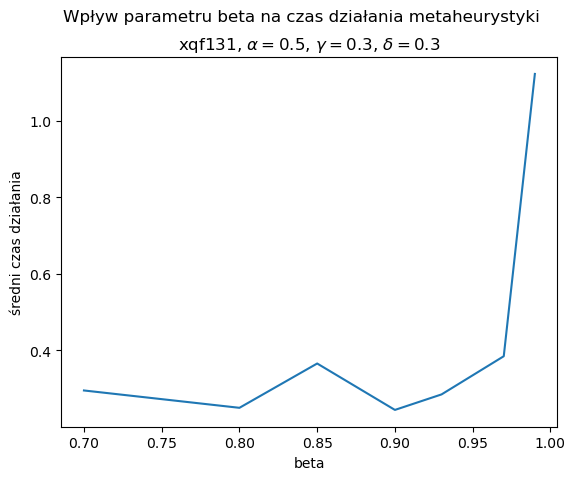
\includegraphics[height=9.5cm]{../../plots/sa-tuning-beta-time-xqf131.png}
    \end{figure}
    
    \begin{figure}[h!]
        \centering
        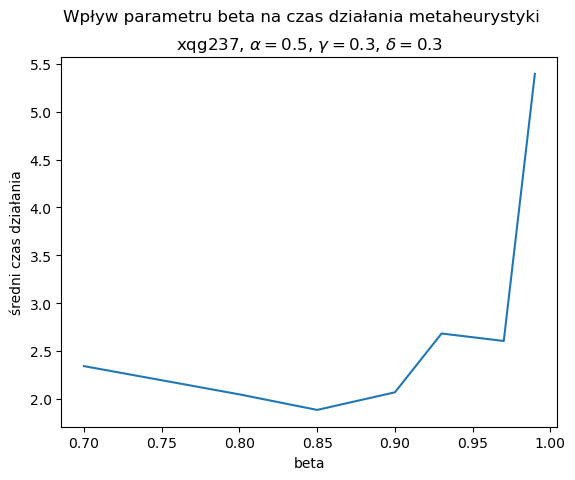
\includegraphics[height=9.5cm]{../../plots/sa-tuning-beta-time-xqg237.png}
    \end{figure}

\newpage

\subsubsection{Wpływ zmiany długości epoki i liczby iteracji bez poprawy na średnią długośc cyklu rozwiązania}
    \begin{figure}[h!]
        \centering
        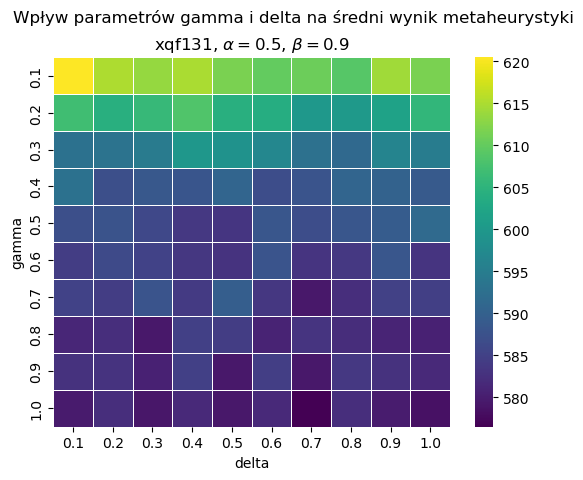
\includegraphics[height=10.0cm]{../../plots/sa-tuning-gamma-delta-avg-xqf131.png}
    \end{figure}

    \begin{figure}[h!]
        \centering
        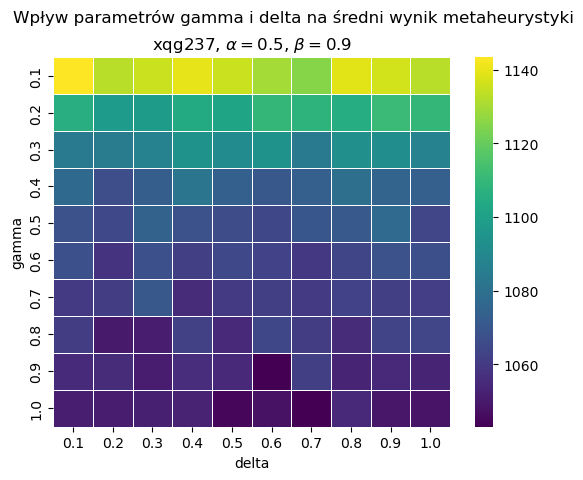
\includegraphics[height=10.0cm]{../../plots/sa-tuning-gamma-delta-avg-xqg237.png}
    \end{figure}

\newpage

\subsubsection{Wpływ zmiany długości epoki i liczby iteracji bez poprawy na minimalną długośc cyklu rozwiązania}
    \begin{figure}[h!]
        \centering
        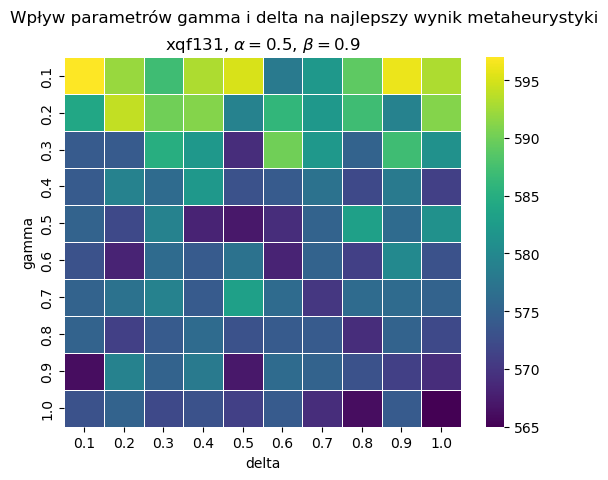
\includegraphics[height=10.0cm]{../../plots/sa-tuning-gamma-delta-min-xqf131.png}
    \end{figure}

    \begin{figure}[h!]
        \centering
        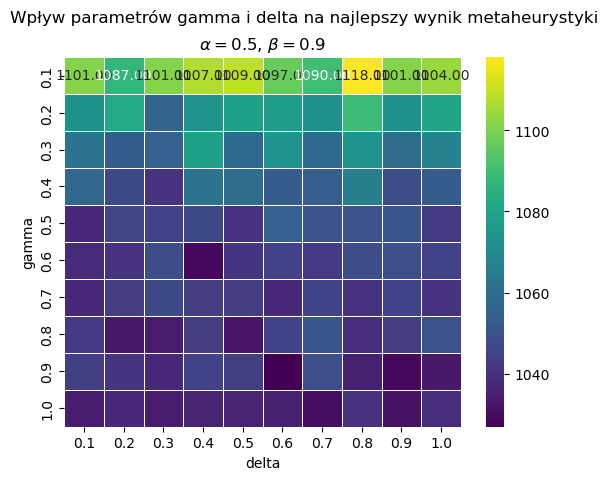
\includegraphics[height=10.0cm]{../../plots/sa-tuning-gamma-delta-min-xqg237.png}
    \end{figure}
\newpage

\subsubsection{Wpływ zmiany długości epoki i liczby iteracji bez poprawy na średni czas działania heurystyki}
    \begin{figure}[h!]
        \centering
        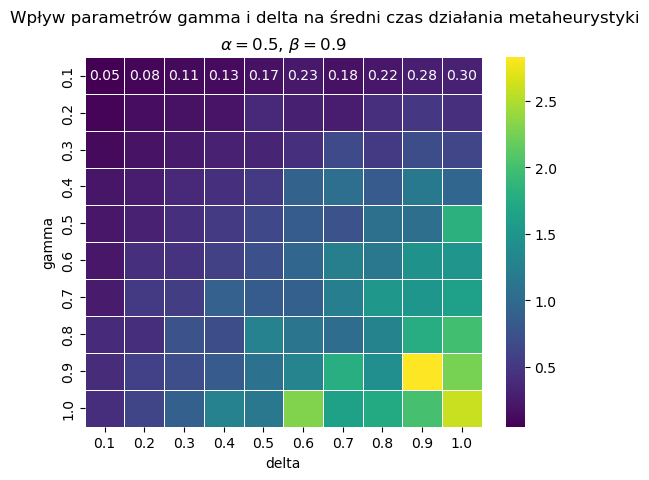
\includegraphics[height=10.0cm]{../../plots/sa-tuning-gamma-delta-time-xqf131.png}
    \end{figure}

    \begin{figure}[h!]
        \centering
        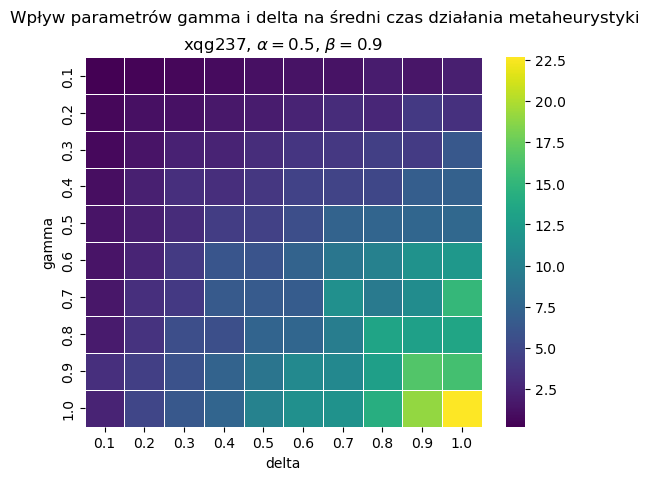
\includegraphics[height=10.0cm]{../../plots/sa-tuning-gamma-delta-time-xqg237.png}
    \end{figure}

\newpage

\subsection{Tabu Search}

\subsubsection{Wpływ zmiany długości listy tabu oraz liczby iteracji bez poprawy na średnią długośc cyklu rozwiązania}
    \begin{figure}[h!]
        \centering
        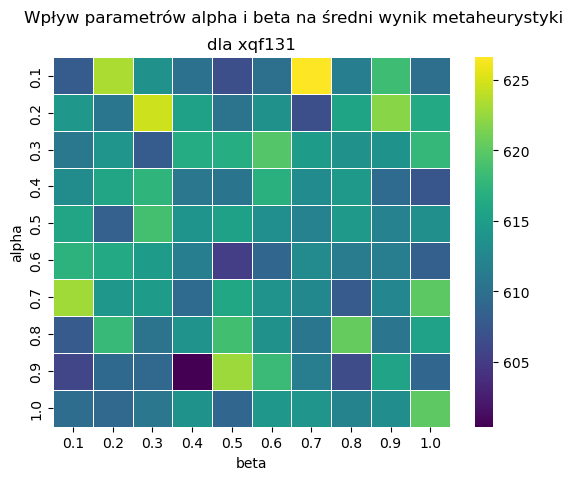
\includegraphics[height=9cm]{../../plots/ts-tuning-alpha-beta-avg-xqf131.png}
    \end{figure}
    
    \begin{figure}[h!]
        \centering
        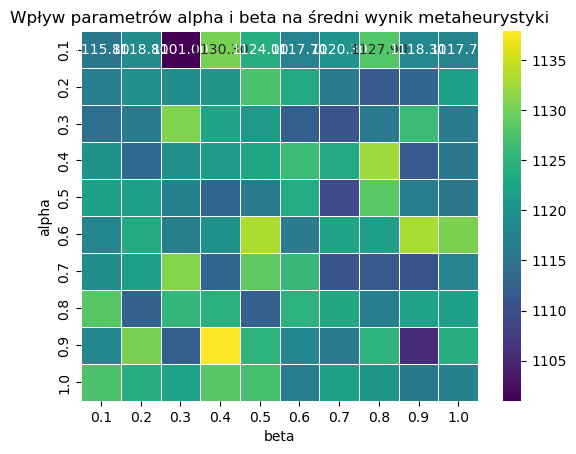
\includegraphics[height=9cm]{../../plots/ts-tuning-alpha-beta-avg-xqg237.png}
    \end{figure}

\newpage

\subsection{Wpływ zmiany długości listy tabu oraz liczby iteracji bez poprawy na minimalną długośc cyklu rozwiązania}
    \begin{figure}[h!]
        \centering
        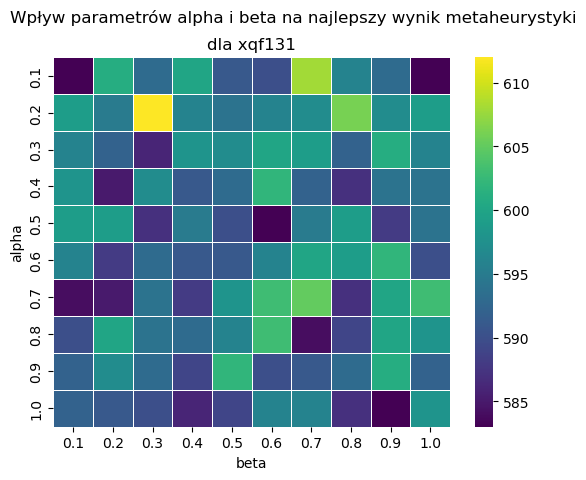
\includegraphics[height=9cm]{../../plots/ts-tuning-alpha-beta-min-xqf131.png}
    \end{figure}
    
    \begin{figure}[h!]
        \centering
        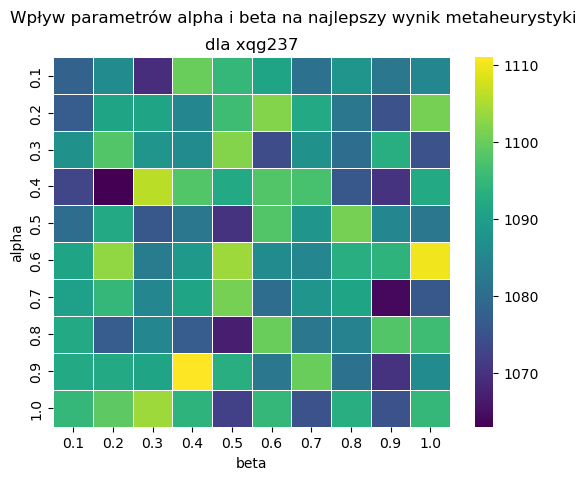
\includegraphics[height=9cm]{../../plots/ts-tuning-alpha-beta-min-xqg237.png}
    \end{figure}

\newpage

\subsection{Wpływ zmiany długości listy tabu oraz liczby iteracji bez poprawy na średni czas działania heurystyki}
    \begin{figure}[h!]
        \centering
        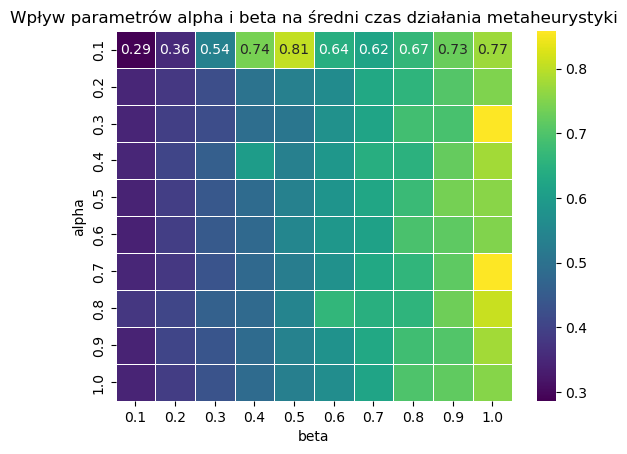
\includegraphics[height=9cm]{../../plots/ts-tuning-alpha-beta-time-xqf131.png}
    \end{figure}
    
    \begin{figure}[h!]
        \centering
        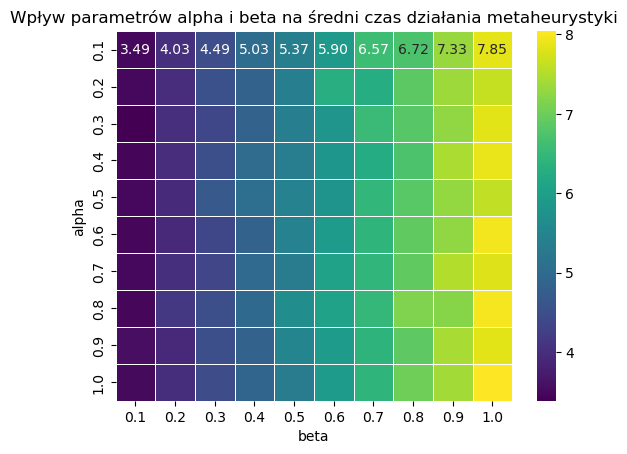
\includegraphics[height=9cm]{../../plots/ts-tuning-alpha-beta-time-xqg237.png}
    \end{figure}

\newpage

\subsubsection{Wpływ rozwiązania początkowego i metody generowania otoczenia na średnią dlugość cyklu}
\begin{table}[h!]
    \centering
    \begin{tabular}{|c|c|c|c|c|}
        \hline 
        \multirow{2}{*}{Przykład} & \multicolumn{2}{|c|}{Losowe rozwiązania początkowe} & \multicolumn{2}{|c|}{Rozwiązanie początkowe bazujące na MST} \\
        \cline{2-5}
        \cline{2-5} & Otoczenie pełne & Otoczenie losowe & Otoczenie pełne & Otoczenie losowe \\
        \hline
        xqf131 & 610 & 640 & 602 & 620 \\
        \hline
        xqg237 & 1116 & 1166 & 1089 & 1132 \\
        \hline
        pma343 & 1487 & 1535 & 1454 & 1503 \\
        \hline
    \end{tabular}
\end{table}

\subsubsection{Wpływ rozwiązania początkowego i metody generowania otoczenia na minimalną dlugość cyklu}
\begin{table}[h!]
    \centering
    \begin{tabular}{|c|c|c|c|c|}
        \hline 
        \multirow{2}{*}{Przykład} & \multicolumn{2}{|c|}{Losowe rozwiązania początkowe} & \multicolumn{2}{|c|}{Rozwiązanie początkowe bazujące na MST} \\
        \cline{2-5}
        \cline{2-5} & Otoczenie pełne & Otoczenie losowe & Otoczenie pełne & Otoczenie losowe \\
        \hline
        xqf131 & 582 & 593 & 594 & 594 \\
        \hline
        xqg237 & 1070 & 1118 & 1060 & 1085 \\
        \hline
        pma343 & 1433 & 1474 & 1428 & 1455 \\
        \hline
    \end{tabular}
\end{table}

\subsubsection{Wpływ rozwiązania początkowego i metody generowania otoczenia na średni czas działania heurystyki}
\begin{table}[h!]
    \centering
    \begin{tabular}{|c|c|c|c|c|}
        \hline 
        \multirow{2}{*}{Przykład} & \multicolumn{2}{|c|}{Losowe rozwiązania początkowe} & \multicolumn{2}{|c|}{Rozwiązanie początkowe bazujące na MST} \\
        \cline{2-5}
        \cline{2-5} & Otoczenie pełne & Otoczenie losowe & Otoczenie pełne & Otoczenie losowe \\
        \hline
        xqf131 & 0.18 & 0.007 & 0.06 & 0.004 \\
        \hline
        xqg237 & 1.9 & 0.03 & 0.5 & 0.02 \\
        \hline
        pma343 & 7.4 & 0.13 & 2.1 & 0.07 \\
        \hline
    \end{tabular}
\end{table}

\section{Dobór parametrów}
\subsection{Symulowane wyżarzanie}
\begin{itemize}
    \item Temperatura początkowa: $\alpha = 0.5$
    \item Chłodzenie: $\beta = 0.95$
    \item Długość epoki: $\gamma = 0.2$
    \item Liczba iteracji bez poprawy: $\delta = 0.1$
    \item Typ otoczenia: \texttt{INVERT}
    \item Wybór otoczenia: pełne
    \item Rozwiązanie początkowe: losowe
\end{itemize}

\subsection{Tabu Search}
\begin{itemize}
    \item Długość listy tabu: $\alpha = 0.1$
    \item Liczba iteracji bez poprawy: $\beta = 0.2$
    \item Typ otoczenia: \texttt{INVERT}
    \item Wybór otoczenia: pełne
    \item Rozwiązanie początkowe: oparte o MST
\end{itemize}

\newpage

\section{Wyniki}

\begin{table}[h!]
    \centering
    \begin{tabular}{|c|c|c|c|c|c|c|c|}
        \hline
        \multirow{2}{*}{Przykład} & \multirow{2}{*}{Optimum} & \multicolumn{2}{|c|}{Local Search} & \multicolumn{2}{|c|}{Sumulowane Wyżarzanie}  & \multicolumn{2}{|c|}{Tabu Search}  \\
        \cline{3-8}
        & & śr. waga & min. waga & śr. waga & min. waga & śr. waga & min. waga \\
        \hline
        xqf131 & 564 & 612 & 578 & 580.8 & 567 & 602.4 & 594 \\
        \hline
        xqg237 & 1019 & 1115.8 & 1062 & 1056 & 1036 & 1089 & 1060 \\
        \hline
        pma343 & 1368 & 1484.7 & 1424 & 1395.2 & 1378 & 1454.0 & 1428 \\
        \hline
        pka379 & 1332 & 1445.9 & 1399 & 1380.6 & 1360 & 1398.8 & 1376 \\
        \hline
        bcl380 & 1621 & 1817.5 & 1728 & 1730.4 & 1685 & 1750 & 1707 \\
        \hline
        pbl395 & 1281 & 1429.0 & 1359 & 1363.8 & 1317 & 1377.8 & 1352 \\
        \hline
        pbk411 & 1343 & 1488.5 & 1426 & 1431.9 & 1397 & 1433.3 & 1405 \\
        \hline
        pbn423 & 1365 & 1521.6 & 1454 & 1457.6 & 1412 & 1468.4 & 1440 \\
        \hline
        pbm436 & 1443 & 1612.0 & 1535 & 1540.2 & 1481 & 1563.5 & 1535 \\
        \hline
        xql662 & 2513 & 2813.3 & 2707 & 2682.5 & 2617 & 2699.4 & 2673 \\
        \hline
        xit1083 & 3558 & 4021.2 & 3919 & 3825.5 & 3746 & 3909.11 & 3768 \\
        \hline
        icw1483 & 4416 & 4990.5 & 4839 & 4731.1 & 4628 & 4739.7 & 4733 \\
        \hline
        djc1785 & 6115 & 6872.1 & 6697 & 6545.1 & 6460 & 6470.7 & 6450 \\
        \hline
        dcb2086 & 6600 & 7457.8 & 7313 & 7129.6 & 7074 & 7171.7 & 7153 \\
        \hline
        pds2566 & 7643 & 8701.8 & 8506 & 8225 & 8151 & 8377 & 8255 \\
        \hline
    \end{tabular}
    \caption{Porównanie wyników metaheurystyk: Local Search, Symulowane Wyżarzanie oraz Tabu Search.}
\end{table}

\newpage

% \section{Wizualizacje rozwiązań}
% \def \myArray{xqf131, xqg237, pma343, pka379, bcl380, pbl395, pbk411, pbn423, pbm436, xql662, xit1083, icw1483, djc1785, dcb2086, pds2566}

% \foreach \text in \myArray {
%     \subsection{\text}

%     \begin{figure}[h!]
%         \centering
%         \includegraphics[height=5.0cm]{../../plots/\text-ls-imp.png}
%     \end{figure}
    
%     \begin{figure}[h!]
%         \centering
%         \includegraphics[height=5.0cm]{../../plots/\text-tsp-mst.png}
%     \end{figure}

%     \begin{figure}[h!]
%         \centering
%         \includegraphics[height=5.0cm]{../../plots/\text-tsp-ls-mst.png}
%     \end{figure}

%     \begin{figure}[h!]
%         \centering
%         \includegraphics[height=5.0cm]{../../plots/\text-tsp-ls-mst-stats.png}
%     \end{figure}

%     \newpage

%     \begin{figure}[h!]
%         \centering
%         \includegraphics[height=5.0cm]{../../plots/\text-tsp-ls-rand.png}
%     \end{figure}

%     \begin{figure}[h!]
%         \centering
%         \includegraphics[height=5.0cm]{../../plots/\text-tsp-ls-rand-stats.png}
%     \end{figure}

%     \begin{figure}[h!]
%         \centering
%         \includegraphics[height=5.0cm]{../../plots/\text-tsp-ls-rand-rand.png}
%     \end{figure}

%     \begin{figure}[h!]
%         \centering
%         \includegraphics[height=5.0cm]{../../plots/\text-tsp-ls-rand-rand-stats.png}
%     \end{figure}

%     \newpage
% }

\end{document}
